\chapter[Formulation du problème de propagation d'interfaces régulières \piecewise\ en \troisD]{Formulation mathématique du problème de propagation d'interfaces régulières \piecewise\ en trois dimensions}
\chaptermark{Formulation du problème de propagation d'interfaces $\contgeom{1}$ \piecewise\ en \troisD}
\label{chap:formulation_probleme_propagation}

Objectif : définir/caractériser une surface poser le problème

On considère une interface $\Sigma$ entre deux milieux distincts (\eg un solide et un fluide).
Dans cette thèse, on se concentre sur des problèmes en trois dimensions. 
$\Sigma$ représente donc une surface (\ie une variété de dimension 2) que l’on supposera orientable et fermée.
De cette manière, $\Sigma$ sépare l'espace en un domaine \textit{intérieur} $\Omega$ (que l'on supposera ouvert) et un domaine \textit{extérieur} $\complement{\Omega}$.
Avant de rentrer dans le vif du sujet --- à savoir la propagation de l'interface $\Sigma$ --- on rappelle les bases de la géométrie différentielle des surfaces et plus particulièrement des surfaces régulières par morceaux.


\section{Géométrie différentielle des courbes et surfaces?}
courbes et surfaces paramétriques : vocabulaire (arc, carreau, espace et domaine paramétriques, carreau restreint, courbes de restriction),  vecteur(s) et plan tangents, vecteur (pseudo-)normal, tenseur métrique, première et seconde formes fondamentales, courbures principales, gaussienne et moyenne
\par
notion de continuités paramétrique/géométrique

\section{Caractérisation d'une surface régulière \piecewise}
décomposition en nappes régulières ($\contgeom{1}$), courbes singulières (crêtes?) et points irréguliers (coins?) (\cf notes Huygens)
\par\bigskip
(Inspiré par \cite[p.65]{rossignac1985} et \cite[Section 2.6]{rossignac1986}.)\par

\begin{figure}
	\centering
	\setlength{\imagewidth}{80mm}%
\setlength{\imageheight}{\imagewidth}%
\DTLsetseparator{,}%
\DTLloaddb[noheader,keys={x,y,a}]{dbcorners}{figures/data/piecewise_smooth_surface/corners_xya.dat}%
\DTLloaddb[noheader,keys={x,y,a}]{dbedgemidp}{figures/data/piecewise_smooth_surface/edge_midpoints_xya.dat}%
\begin{tikzpicture}[%
		x=\imagewidth, y=\imageheight,
		img/.style={anchor=south west, inner sep=0},
		anot/.style={-{Latex[length=4pt]}, shorten >=2pt},
		anotpoint/.style={anot, shorten >=5pt},
	]
	%%% SURFACE
	\node[img] at (0,0) {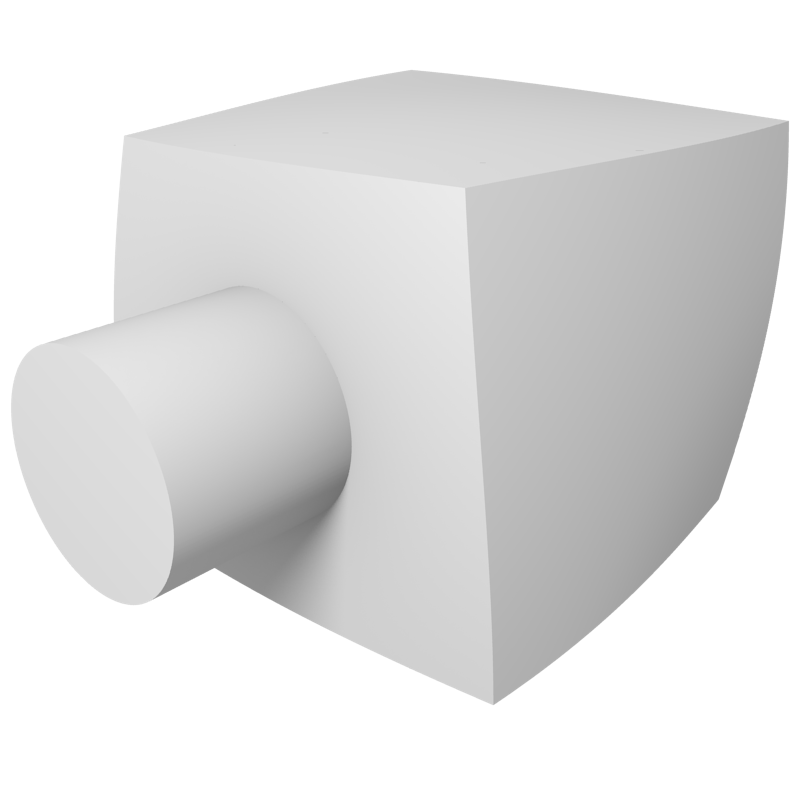
\includegraphics[width=\imagewidth]{piecewise_smooth_surface/surface}};
	%%% HIDDEN EDGES
	\node[img] at (0,0) {
\includegraphics[width=\imagewidth]{piecewise_smooth_surface/edges_hidden}};
	%%% HIDDEN CORNERS
	\DTLforeach*{dbcorners}{\locx=x, \locy=y, \loca=a}{%
		\ifnum \loca = 0
			\fill[black] (\locx,\locy) circle (1.0pt);
		\fi
	}%
	%%% SURFACE (semi-transparent to mask hidden edges & corners)
	{\transparent{0.75}
		\node[img] at (0,0) {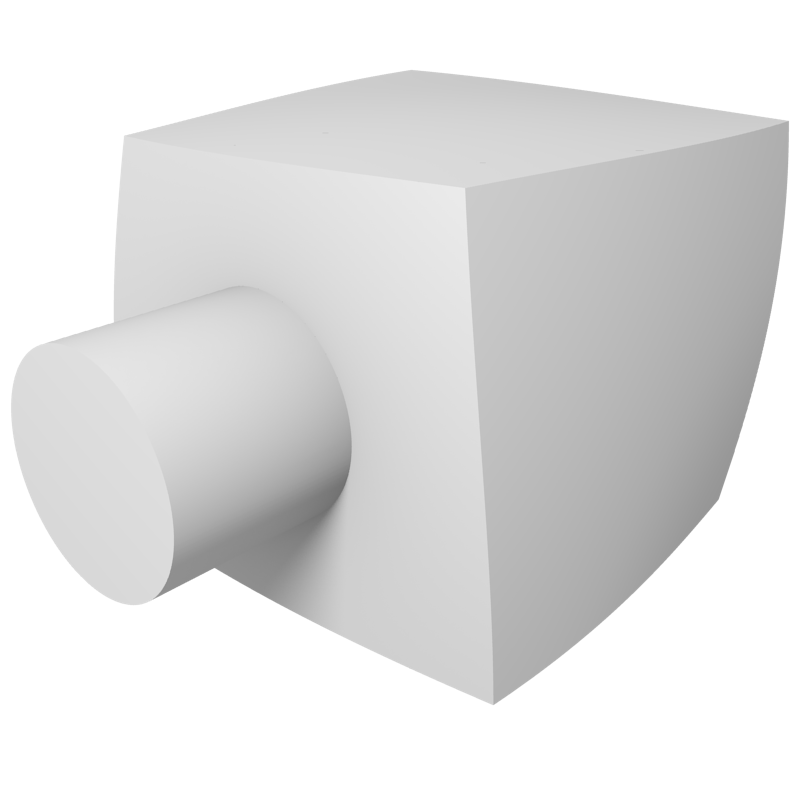
\includegraphics[width=\imagewidth]{piecewise_smooth_surface/surface}};
	}%
	%%% VISIBLE EDGES
	\node[img] at (0,0) {
\includegraphics[width=\imagewidth]{piecewise_smooth_surface/edges_visible}};
	%%% VISIBLE CORNERS
	\DTLforeach*{dbcorners}{\locx=x, \locy=y, \loca=a}{%
		\ifnum \loca = 1
			\fill[black] (\locx,\locy) circle (1.2pt);
		\fi
	}%
	%
	%%% ANOTATIONS
	\DTLassign{dbcorners}{6}{\locxa=x,\locya=y,\loca=a}% 	
	\DTLassign{dbcorners}{4}{\locxb=x,\locyb=y,\loca=a}% 
	\DTLassign{dbcorners}{1}{\locxc=x,\locyc=y,\loca=a}% 
	%\node[anchor=west] (anotSingPts) at (\locxb,{0.5*(\locya + \locyb)}) {points singuliers};
	\node[anchor=east] (anotSingPts) at (1.2,0.2) {coins};
	\draw[anot] (anotSingPts) to [bend left=10] (\locxa, \locya);
	\draw[anot] (anotSingPts) to [bend right=20] (\locxb, \locyb);
	\draw[anot] (anotSingPts) to [bend right=10] (\locxc, \locyc);
	%
	\DTLassign{dbedgemidp}{19}{\locxa=x,\locya=y,\loca=a}% 	
	\DTLassign{dbedgemidp}{7}{\locxb=x,\locyb=y,\loca=a}% 
	\DTLassign{dbedgemidp}{14}{\locxc=x,\locyc=y,\loca=a}% 
	\node[anchor=west] (anotSingCurv) at (-0.2,0.9) {crêtes};
	\draw[anot] (anotSingCurv) to [bend right=10] (\locxa, \locya);
	\draw[anot] (anotSingCurv) to [bend right=40] (\locxb, \locyb);
	\draw[anot] (anotSingCurv.east) to [bend left=10] (\locxc, \locyc);
\end{tikzpicture}
\DTLgdeletedb{dbcorners}%
\DTLgdeletedb{dbedgemidp}%

	\caption{Surface régulière par morceaux dont les courbes et points singuliers sont mis en évidence.}
	\label{fig:piecewise_smooth_surface_decomposition}
\end{figure}

La frontière $\boundary{\Omega}$ du solide $\Omega$ est une surface de continuité $\contgeom{1}$ (\ie possède une direction normale continue) par morceaux. 
Les singularités géométriques de $\boundary{\Omega}$ peuvent être de dimension 1 (courbes) ou 0 (points).
Les courbes singulières de $\boundary{\Omega}$ sont elle-mêmes des variétés différentielles de continuité $\contgeom{1}$ (\ie possède une direction tangente continue) excepté aux points singuliers.


\section{Formulation lagrangienne du problème de propagation d'interface}
[EDP avec vecteur vitesse ou vitesse normale, problème de définition au niveau des courbes singulières et points irréguliers]
\par\bigskip
La formulation lagrangienne traditionnelle du problème de propagation d'interface consiste à exprimer l'évolution de la position d'un point $\bx \in \Sigma$ comme une équation différentielle
\begin{equation}
	\frac{\partial \bx}{\partial t} = \vrm{u}(\bx,t).
	\label{eq:lagrange_vecteur_vitesse}
\end{equation}
La composante tangentielle du vecteur vitesse n'affecte pas la forme de l'interface. 
En principe, on peut donc formuler de façon équivalente la propagation de $\Sigma$ suivant un champ de vitesse normale $\nu : \Sigma \times \reals_+ \to \reals$
\begin{equation}
	\frac{\partial \bx}{\partial t} = \nu(\bx,t) \unv(\bx,t),
	\label{eq:lagrange_vitesse_normale}
\end{equation}
où $\unv(\bx,t)$ désigne la direction normale à $\Sigma$ en $\bx$ à l'instant $t$.
\par






\section{Principe de Huygens avec condition d'entropie}
\label{section:principe_huygens}
[Histoire, formulation, notion d'enveloppe de sphères/boules, construction géométrique au lieu de EDP, définitions implicites (\cf notes Huygens)]
\par\bigskip

Dans la suite, étant donné un sous-ensemble (ouvert ou fermé) $E$ de $\reals^d$, on notera $\complement{E} := \reals^d \setminus E$ son \textit{complémentaire}, $\boundary{E}$ sa \textit{frontière}, $\interior{E}$ son \textit{intérieur} et $\closure{E} = E \cup \boundary{E}$ son \textit{adhérence}.
\par\bigskip

\def\p{\vit{p}}
\def\q{\vit{q}}
Soient $r> 0$ et $\p$ un point de $\reals^3$. 
On note $\sphere{\p}{r}$ la sphère de rayon $r$ centrée en $\p$
\begin{equation}
    \sphere{\p}{r} := \left\{ 
        \bx \in \reals^3 \mid \normtwo{\bx - \p} = r
    \right\},
\end{equation}
et $\ball{\p}{r}$ la boule \textit{ouverte} de rayon $r$ centrée en $\p$
\begin{equation}
    \ball{\p}{r} := \left\{ 
        \bx \in \reals^3 \mid \normtwo{\bx - \p} < r
    \right\}.
\end{equation}

Soit $\rho : \Sigma \to \reals_{+*}$ une fonction $\alpha$-lipschitzienne sur $\Sigma$ et à valeurs strictement positives. 
On note $\ball{\Sigma}{\rho}$ la réunion des boules centrées sur $\Sigma$ et de rayon $\rho$
\begin{equation}
    \ball{\Sigma}{\rho} := \bigcup_{\p \in \Sigma} \ball{\p}{\rho(\p)}
    = \left\{
        \bx \in \reals^3 \mid \exists \p \in \Sigma \mid \normtwo{\bx - \p} < \rho(\p)
    \right\}.
\end{equation}

Son complémentaire est
\begin{equation}
    \complement{\ball{\Sigma}{\rho}} = \bigcap_{\p \in \Sigma} \complement{\ball{\p}{\rho(\p)}}
    = \left\{
        \bx \in \reals^3 \mid \forall \p \in \Sigma, \normtwo{\bx - \p} \geq \rho(\p)
    \right\},
\end{equation}

et sa frontière est
\begin{align}
    \boundary{\ball{\Sigma}{\rho}} 
    &= \boundary{ \left(\complement{\ball{\Sigma}{\rho}}\right) } ,\nonumber\\
    &= \closure{\ball{\Sigma}{\rho}} \cap 
        \closure{ \left(\complement{\ball{\Sigma}{\rho}}\right) } ,\nonumber\\
%    &= \left\{
%        \bx \in \reals^3 
%        \mid \forall \p \in \Sigma, \normtwo{\bx - \p} \geq \rho(\p) 
%        \text{ et }
%        \exists \p \in \Sigma \mid \normtwo{\bx - \p} \leq \rho(\p)
%    \right\} ,\nonumber\\
     &= \left\{
        \bx \in \reals^3 
        \mid \forall \p \in \Sigma, \normtwo{\bx - \p} \geq \rho(\p) 
        \text{ et }
        \exists \p \in \Sigma \mid \normtwo{\bx - \p} = \rho(\p)
    \right\}.
\end{align}

\par\bigskip

On note $\dilation{\Omega}{\rho}$ la \guillemets{dilatation} de $\Omega$ par $\rho$
\begin{equation}
    \dilation{\Omega}{\rho} = \Omega \cup \ball{\Sigma}{\rho}.
\end{equation}

On note $\EoB{\Sigma}{\rho}$ sa frontière
\begin{align}
    \EoB{\Sigma}{\rho} 
    &:= \boundary{ \!\left(\dilation{\Omega}{\rho}\right) }, \\
    &=  \boundary{ \!\left(\complement{ \left(\dilation{\Omega}{\rho}\right) }\right) } , \nonumber\\
    &=  \boundary{ \!\left(\complement{\Omega} \cap \complement{\ball{\Sigma}{\rho}}\right) },\nonumber\\
    &= 
    \left\{
        \bx \in \interior{ \left(\complement{ \Omega }\right) }
        \mid \forall \q \in \Sigma, \normtwo{\bx - \q} \geq \rho(\q) 
        \text{ et }
        \exists \p \in \Sigma \mid \normtwo{\bx - \p} = \rho(\p)
    \right\}.
\end{align}
Il s'agit de l'\textit{enveloppe des boules}\footnote{plus exactement des demi-boules à l'extérieur de $\Omega$.} (EdB) centrées sur $\Sigma$ et de rayon $\rho$.

\clearpage
\section{Représentation par les frontières}
Origine, utilisation, concept, définitions formelles des entités, lien avec la décomposition d'une surface $\contgeom{1}$ \piecewise, (géométrie différentielle des courbes et surfaces paramétriques), structures de données (DCEL)

\begin{figure}
	\centering
	\colorlet{topo_color}{mycolor_5}
\colorlet{orient_color}{topo_color!60!mycolor_2}
\colorlet{group_color}{topo_color!40!mycolor_3}
\colorlet{geom_color}{mycolor_1}%{mycolor_3}
\def\bigsep{5mm}
\def\smallsep{2.5mm}
\pgfdeclarelayer{bg}    % declare background layer
\pgfsetlayers{bg,main}  % set the order of the layers (main is the standard layer)
\begin{tikzpicture}[
	x = 30mm,
	y = 9.75mm,
	arrow/.style={thick, -stealth', shorten <= 2pt, shorten >= 2pt},
	bounded/.style={arrow, dash pattern=on 4pt off 2pt},
	described/.style={arrow},
	composed/.style={arrow, dash pattern=on 1.5pt off 1.5pt},
	box/.style={rectangle, rounded corners=0.8ex},
	number/.style={font=\footnotesize},
	topo/.style={fill=topo_color!33!white},
	geom/.style={fill=geom_color!33!white},
	orient/.style={fill=orient_color!33!white},
	group/.style={fill=group_color!33!white},
	type/.style={font=\bfseries},%, anchor=east},
	label/.style={anchor=west, inner sep=2pt, font=\scriptsize},
	class/.style={dotted, thick, line cap=round},
	bigclass/.style={class, rounded corners=\bigsep, dash pattern=on 0.8pt off 3.2pt},
	smallclass/.style={class, rounded corners=\smallsep, dash pattern=on 0.3pt off 2.8pt},
	]
	% entités topologiques
	\node[box, topo] at (-1,1) (volume) {Solide};
	\node[box, topo] at (0,1) (face) {Face};
	\node[box, topo] at (1,1) (edge) {Arête};
	\node[box, topo] at (2,1) (vertex) {Sommet};
	% entités de groupement
	\node[box, group] at (-1,3) (shell) {Coquille};
	\node[box, group] at (0,3) (wire) {Contour};
	% entités d'orientation
	\node[box, orient] at (1,3) (halfedge) {Co-arête};
	% entités géométriques
	\node[box, geom] at (0,-1) (surface) {Surface};
	\node[box, geom] at (1,-1) (curve) {Courbe};
	\node[box, geom] at (2,-1) (point) {Point};
	%
	% relations "décrit par"
	\draw[described] (face) -- (surface);
	\draw[described] (edge) -- (curve);
	\draw[described] (vertex) -- (point);
	% relations "délimité par"
	\draw[bounded] (volume) -- 
		node[number,left]{$1+n_{\mathrm{s}}^{\mathrm{int}}$} 
		(shell);
	\draw[bounded] (face) -- 
		node[number,right]{$1+n_{\mathrm{w}}^{\mathrm{int}}$} 
		(wire);
	\draw[bounded] (edge) -- node[number,above]{$2$} (vertex);
	% relations "composé de"
	\draw[composed] (shell) -- node[number,above right]{$n$} (face);
	\draw[composed] (wire) -- node[number,above]{$n$} (halfedge);
	\draw[composed] (edge) -- node[number,right]{$2$} (halfedge);
	%
	% noms de classes
	\gettikzxy{(current bounding box.east)}{\xbbE}{\ybbE}%
	\node[type, geom_color!90!gray] (geomet) at (-1,-1) {Géométrie};
	\node[type, anchor=east, orient_color!90!gray] (orientation) at ({\xbbE-0.5*\smallsep},3) {Orientation};
	\gettikzxy{(halfedge.east)}{\xhE}{\yhE}%
	\gettikzxy{(orientation.west)}{\xoW}{\yoW}%
	\gettikzxy{(shell.west)}{\xsW}{\ysW}%
	\node[type, anchor=east, group_color!90!gray] (grouping) at ({\xsW-\xoW+\xhE},3) {Groupement};
	\gettikzxy{(grouping.west)}{\xgrW}{\ygrW}%
	\gettikzxy{(grouping.south)}{\xgrS}{\ygrS}%
	\gettikzxy{(volume.south)}{\xvS}{\yvS}%
	\node[type, anchor=west, topo_color!90!gray] (topology) at (\xgrW,{0.5*(\ygrS-\smallsep + \yvS-\bigsep)}) {Topologie};
	%
	% classes
	\gettikzxy{(vertex.south east)}{\xtSE}{\ytSE}%
	\gettikzxy{(shell.north)}{\xtN}{\ytN}%
	\gettikzxy{(grouping.west)}{\xtW}{\ytW}%
	\gettikzxy{(geomet.west)}{\xgeW}{\ygeW}%
	\gettikzxy{(topology.north)}{\xtM}{\tmp}%
	\gettikzxy{(grouping.south)}{\tmp}{\ytM}%
	\gettikzxy{(halfedge.south west)}{\xoSW}{\yoSW}%
	\gettikzxy{(halfedge.north)}{\xoN}{\yoN}%
	\gettikzxy{(orientation.north east)}{\xoNE}{\yoNE}%
	\gettikzxy{(grouping.south west)}{\xgrSW}{\ygrSW}%
	\gettikzxy{(wire.south)}{\xgrS}{\ygrS}%
	\gettikzxy{(wire.north east)}{\xgrNE}{\ygrNE}%
	\gettikzxy{(surface.south)}{\xgeS}{\ygeS}%
	\gettikzxy{(surface.north)}{\xgeN}{\ygeN}%
	\begin{pgfonlayer}{bg}    % select the background layer
		\draw[bigclass, topo_color, fill=topo_color!8!white] 
		({\xtSE+\bigsep},{\ytSE-\bigsep}) --
		({\xtSE+\bigsep},{\ytN+\bigsep}) --
		({\xtW-\bigsep},{\ytN+\bigsep}) --
		({\xtW-\bigsep},{\ytSE-\bigsep}) -- cycle;
		%
		\draw[smallclass, orient_color, fill=orient_color!8!white] 
		({\xoSW-\smallsep},{\yoSW-\smallsep}) -- 
		({\xoNE+\smallsep},{\yoSW-\smallsep}) -- 
		({\xoNE+\smallsep},{\yoN+\smallsep}) -- 
		({\xoSW -\smallsep},{\yoN+\smallsep}) -- cycle;
		%
		\draw[smallclass, group_color, fill=group_color!8!white] 
		({\xgrSW-\smallsep},{\ygrS-\smallsep}) -- 
		({\xgrNE+\smallsep},{\ygrS-\smallsep}) -- 
		({\xgrNE+\smallsep},{\ygrNE+\smallsep}) -- 
		({\xgrSW -\smallsep},{\ygrNE+\smallsep}) -- cycle;
		%
		\draw[bigclass, geom_color, fill=geom_color!8!white]
		({\xgeW-\bigsep},{\ygeS-\bigsep}) -- 
		({\xtSE+\bigsep},{\ygeS-\bigsep}) -- 
		({\xtSE+\bigsep},{\ygeN+\bigsep}) -- 
		({\xgeW-\bigsep},{\ygeN+\bigsep}) -- cycle;
	\end{pgfonlayer}
	% légende des relations
	\coordinate (lgd) at ({\xtW-\bigsep+2pt},{0.5*(\ygeS+\ygeN)});
	\foreach \i in {0,1,2}{
		\coordinate (L\i) at ([yshift={-(\i-1)*2.8ex}]lgd);
		\coordinate (R\i) at ([xshift=7.5mm]L\i);
	}
	\draw[described] (L0) -- (R0) node[label] (lbl0) {décrit par};
	\draw[bounded]   (L1) -- (R1) node[label] (lbl1) {délimité par};
	\draw[composed]  (L2) -- (R2) node[label] (lbl2) {composé de};
	\node[draw=black!25,
	inner sep=2pt,
	rounded corners=\smallsep,
	fit={(L0) (lbl0) (lbl1) (lbl2)}] {};
\end{tikzpicture}
	\caption{Hiérarchie des éléments constituant un modèle \brep.}
	\label{fig:BRep_hierarchy}
\end{figure}

\begin{figure}
	\centering
	\setlength{\imagewidth}{80mm}%
\setlength{\imageheight}{\imagewidth}%
\DTLsetseparator{,}%
\DTLloaddb[noheader,keys={x,y,a}]{dbverts}{figures/data/BRep/verts_xya.dat}%
\begin{tikzpicture}[%
	x=\imagewidth, y=\imageheight,
	img/.style={anchor=south west, inner sep=0}]
	%%%%%%%%%%%%%%%% SHELL %%%%%%%%%%%%%%%%
	%%% FACES
	\node[img] at (0,0) {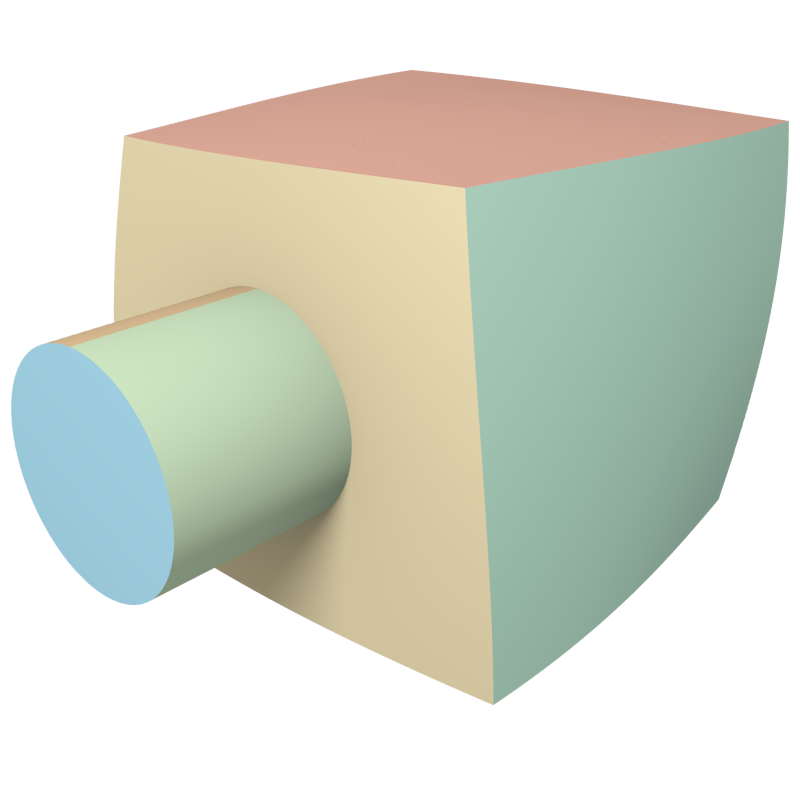
\includegraphics[width=\imagewidth]{BRep/shell}};
	%%% HIDDEN EDGES
	\node[img] at (0,0) {
\includegraphics[width=\imagewidth]{BRep/edges_hidden}};
	%%% HIDDEN VERTICES
	\DTLforeach*{dbverts}{\locx=x, \locy=y, \loca=a}{%
		\ifnum \loca = 0
			\fill[black] (\locx,\locy) circle (1.0pt);
		\fi
	}%
	%%% FACES (semi-transparent to mask hidden edges & verts)
	{\transparent{0.75}
		\node[img] at (0,0) {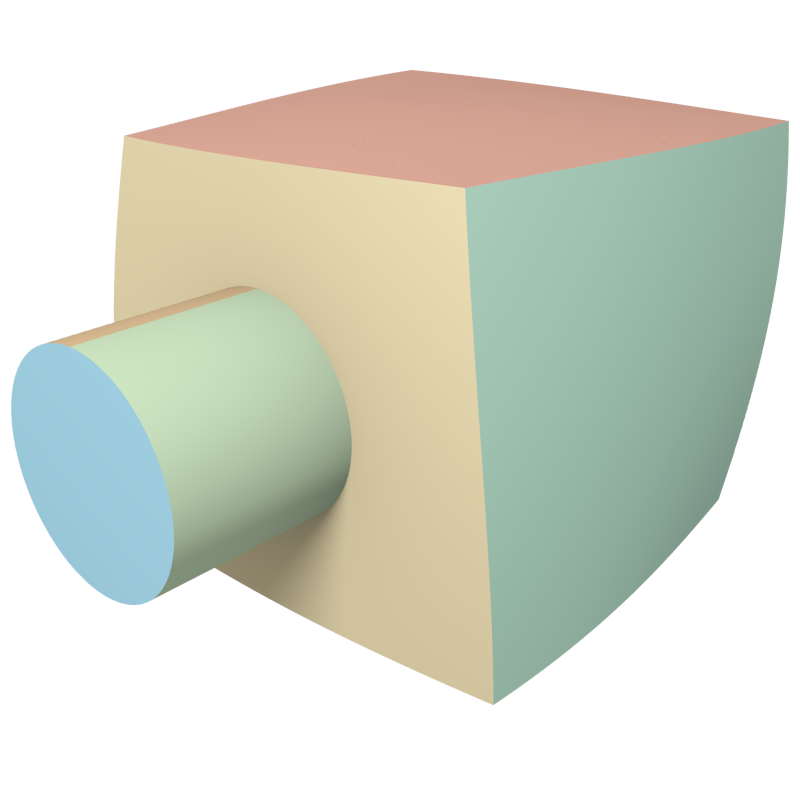
\includegraphics[width=\imagewidth]{BRep/shell}};
	}%
	%%% VISIBLE EDGES
	\node[img] at (0,0) {
\includegraphics[width=\imagewidth]{BRep/edges_visible}};
	%%% VISIBLE VERTICES
	\DTLforeach*{dbverts}{\locx=x, \locy=y, \loca=a}{%
		\ifnum \loca = 1
			\fill[black] (\locx,\locy) circle (1.0pt);
		\fi
	}%
\end{tikzpicture}
\DTLgdeletedb{dbverts}%
%%%%%%%%%%%%%%%%%%%%%%%%%%%%%%%%%%%%%%
%
%%%%%%%%%%%%%%%% FACES %%%%%%%%%%%%%%%%
\def\imfacew{44mm}
\def\ngriduv{6}
\def\vertsep{0.05}
\def\edglabsepuv{0.17}
\def\wirlabsepuv{0.18}
\def\edglabsepxyz{0.06}
\def\iniwclr{0.3}
\def\decwclr{0.3}%{0.2}
\def\uvscale{0.34}
\def\uvyshift{-0.7}
\pgfmathsetmacro\sepyshift{0.5 * (\uvyshift+\uvscale)}%
%
\begin{tikzpicture}[%
	x = \imfacew, y = \imfacew,
	gridtick/.style={red, fill=white, font=\tiny, inner sep=0.5pt},
	img/.style={anchor=south west, inner sep=0},
	label/.style={inner sep=1pt, font=\scriptsize},
	uvgrid/.style={black!10!white},
	curv/.style={line width=0.8pt, line cap=round},
	spacelabel/.style={anchor=north, rotate=90, inner sep=0, font=\bfseries},
	]
	\foreach \jfa/\ifa in {-1/007, 0/008, 1/002}{%
		\figbrepface{\ifa}{{1.05*\jfa - 0.5}}{{-\sepyshift}}%\hfill
	}%
	\draw[very thick, gray, dashed] 
	({-0.5*\textwidth},0) -- ++ 
	(\textwidth,0);
	\node[spacelabel] (xyzspace) at 
	({-0.5*\textwidth},{-\sepyshift+0.5}) {Espace euclidien\vphantom{Espace paramétrique}};
	\node[spacelabel] (uvspace) at 
	({-0.5*\textwidth},{\sepyshift-\uvscale}) {Espace paramétrique\vphantom{Espace euclidien}};
\end{tikzpicture}

	\caption{Modèle \brep.}
	\label{fig:BRep}
\end{figure}

\par 
placer avant Formulation lagrangienne? ou fusionner avec Caractérisation d'une surface régulière \piecewise?
